\documentclass[12pt,a4paper,twoside]{ipb}

% comentar caso seja uma disseração de mestrado
% \usepackage{projei}

\usepackage[english]{babel}
\graphicspath{{./images/}}
\usepackage{listings} % incluir listagens
\usepackage{url} % typeset URL's
\usepackage[colorlinks=true,
                    urlcolor=black, %blue
                    linkcolor=black,
                    citecolor=black, %cor das citações
                    bookmarks=true,
                    pdfstartview=FitH]{hyperref}

% Pode ser usado biblatex
\usepackage[style=ieee,backend=biber]{biblatex}
\addbibresource{lib/refs.bib}

\usepackage{lipsum}

\usepackage{tabulary}

%%%%%%%%%%%%%%%%%%%%%%%%%

\title{Yabi - Yet Another Business Inteligence}

\author{Vitório Miguel Prieto Cilia - 40920}
%\authnum{1}
\secondauthor{Nome do Aluno - Número Mecanográfico}
%\secauthnum{2}

\supervisor{Prof. Albano Alves}
\cosupervisor{Prof. Lúcio Valentin}

% Para definir o ano letivo
\courseyear{2017-2018}

% Para nao mostrar a lista de tabelas
%\tablespagefalse

\makeglossaries
\loadglsentries{acronym}


%http://tex.stackexchange.com/questions/59572/custom-page-numbering-for-appendix
\usepackage{etoolbox}


\begin{document}
	
% Coloca a capa, primeira pagina e outros

\beforepreface

%\cleardoublepage

\prefacesection*{Dedicatória}
%\thispagestyle{empty}

%\lipsum[1]

(Facultativo) Dedico este trabalho a ...

%\vfill
%\pagebreak
%\mbox{}
%\vfill
%\pagebreak

%\cleardoublepage

\prefacesection*{Agradecimentos}
%\thispagestyle{empty}

%\lipsum[1]

Firstly, I would like to thank my friends Daniel Costa Valério, Henrique Pinheiro and Sávio Camacam. Together we formed the HEDANVISA group, not only sharing technical knowledge but also forming long-lasting relations.

I would like to also thank both institutions, \gls{UTFPR} and \gls{IPB} for the opportunity of realizing my masters in the scope of a double degree program.

Special thanks Professor Marcos Silvano for enabling Computer Science students of \gls{UTFPR}, Campo Mourão to apply for this program and to Bruno Mendes for his clarifying explanations in regards to writing this document.

%\vfill
%\pagebreak
%\mbox{}
%\vfill
%\pagebreak


%\cleardoublepage

\prefacesection*{Resumo}
%\thispagestyle{empty}

No contexto do Instituto Politécnico de Bragança durante o período de matrículas, o departamento de serviços informáticos é frequentemente interrompido em busca de questionamentos sobre as informações contidas nas bases de dados da instituição.

Para amenizar isso, o Yabi foi desenvolvido. Esta é uma aplicação Web construida com uma interface de usuário feita no Framework Angular e uma aplicação remota que implementa as funcionalidades necessárias e é escrita em Java com o framework Spring. De maneira geral ela fornece um portal que possibilita os colaboradoes da instituição a ter acesso as informações contidas nas bases de dados sem que seja necessário o conhecimento técnico.

Por fim, considera-se que a aplicação final atende aos requisitos de maneira suficiente para ser considerada útil e ao mesmo tempo fornece uma plataforma para desenvolvimentos futuros.

\mbox{}\linebreak
\noindent {\bf Palavras-chave:} plataforma web, business intelligence, angular, spring boot.


%\vfill
%\pagebreak
%\mbox{}
%\vfill
%\pagebreak

%\cleardoublepage

\prefacesection*{Abstract}
%\thispagestyle{empty}

Direct translation (maximum of 250 words) to English of the section ``Resumo''.

\mbox{}\linebreak
\noindent {\bf Keywords:} direct translation of ``Palavras-chave''

%\vfill
%\pagebreak
%\mbox{}
%\vfill
%%\pagebreak

% Coloca indices
\afterpreface
%\cleardoublepage
%\printglossary[type=\acronymtype,title={Acrónimos}]
\printglossary[type=\acronymtype,title={Siglas}]

\bodystart


% Capitulos do documento
\cleardoublepage
\chapter{Introdução}\label{cap:intro}

O Capítulo \ref{cap:intro} é dedicado a uma introdução ao tema do trabalho, descrevendo as ideias gerais do problema em foco e a sua importância. Devem ainda ser explicitados os objetivos do trabalho, clarificada a estrutura do relatório e indicadas as convenções tipográficas.

\section{Enquadramento}

Deve haver um enquadramento introdutório, que descreva o contexto em que o trabalho se insere, referenciando a proposta original do projeto, que deve constar no primeiro apêndice do documento (ver apêndice \ref{apendice1}).

\section{Objetivos}

Os objetivos do trabalho devem ser apresentados de forma clara e compatível com a proposta original do projeto. Na eventualidade de os objetivos originais terem sido reformulados, devem ser apresentadas as razões objetivas que conduziram a essa reformulação.

Idealmente, deve-se incluir um cronograma do projeto, indicando explicitamente as tarefas realizadas e o tempo dedicado a cada uma. Existindo um cronograma na proposta original do projeto, deverão justificar-se eventuais discrepâncias com o cronograma real.


\section{Estrutura do Documento}

Este modelo de relatório assume que a maioria dos projetos de fim de curso são centrados no desenvolvimento de uma solução informática para um problema. Sendo esse contexto, é apropriada uma estrutura que descreva a análise, conceção e desenvolvimento da solução implementada. Em particular, em projetos de desenvolvimento de software, espera-se que o relatório documente as principais fases do ciclo de desenvolvimento.

Nos casos em que o trabalho corresponde sobretudo à integração e/ou avaliação de componentes pré-existentes, a estrutura do relatório deverá ser adaptada em conformidade, com ênfase na descrição das tecnologias subjacentes, sua articulação e avaliação.

A estrutura efetivamente adotada para o resto do relatório é, normalmente, clarificada nesta secção, usando texto semelhante a: ``O resto do relatório está organizado da seguinte forma: no capítulo 2 descreve-se ...; no capítulo 3 ...; ...; finalmente, o último capítulo  apresenta as conclusões e direções de trabalho futuro.''

\section{Normas de Composição}

Para além de uma organização que reflita o percurso seguido, o relatório deve estar bem formatado e ter aspeto sóbrio, convidando à leitura e fazendo jus ao mérito do trabalho descrito. Neste sentido, apresentam-se de seguida algumas das normas a levar em conta\footnote{Estas normas, assim como este modelo de documento, são compatíveis com o preconizado no "Regulamento da Unidade Curricular de Projecto das Licenciaturas", designadamente no que diz respeito ao relatório do projeto.}.

\subsubsection{Convenções Tipográficas}

Por vezes, opta-se por apresentar as convenções tipográficas seguidas no documento, ou seja, em que circunstâncias se usam texto em \textit{itálico}, \textbf{negrito}, ou de \texttt{espaçamento uniforme} (esta última formatação é normalmente usada para apresentar código fonte), bem como quais as fontes tipográficas usadas, respetivas dimensões, etc.


\subsubsection{Tabelas e Figuras}

Tabelas e figuras devem ser numeradas automaticamente e ter um tamanho equilibrado (nem muito grande, nem muito pequeno), como a Tabela \ref{tab:exemplo_de_tabela} e as Figuras  \ref{fig:exemplo_de_figura}, \ref{fig:exemplo_de_figura2} e \ref{fig:exemplo_de_figura3}.

\begin{table}[htbp]	
	\centering
	{\small
		\begin{tabulary}{\linewidth}{|L|C|R|}	
			\hline 	
			{\bf Nome da Coluna 1} & {\bf Nome da Coluna 2} & {\bf Nome da Coluna 3} \\ 
			\hline 
			conteúdo A & conteúdo B & conteúdo C \\ 
			\hline 
			conteúdo D & conteúdo E & conteúdo F \\ 
			\hline 
		\end{tabulary} 
	}	
	\caption{\small{Exemplo de tabela.}}
	\label{tab:exemplo_de_tabela}
\end{table}


\begin{figure}[htbp]
	\centering
	
\includegraphics[scale=0.75]{images/lion_large}
	\caption{Exemplo de imagem PNG.}
	\label{fig:exemplo_de_figura}
\end{figure}

Sempre que possível, devem-se usar formatos escaláveis (e.g., PDF), como na Figura \ref{fig:exemplo_de_figura2}, e evitar imagens comprimidas (formatos JPG, PNG, GIF, etc.), como na Figura \ref{fig:exemplo_de_figura}.

\begin{figure}[htbp]
	\centering
	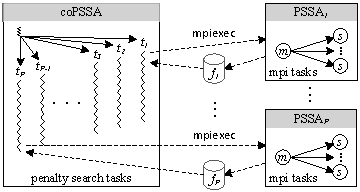
\includegraphics[width=0.75\linewidth]{images/architecture}
	\caption{Exemplo de imagem PDF.}
	\label{fig:exemplo_de_figura2}
\end{figure}


Em gráficos devem-se indicar sempre as grandezas associadas a cada eixo, bem como a respetiva legenda -- ver exemplo na Figura \ref{fig:exemplo_de_figura3}. Adicionalmente, o esquema de cores ou de traços para as linhas, deve ser sóbrio e prevenir ambiguidades na leitura do gráfico.

\begin{figure}[htbp]
	\centering
	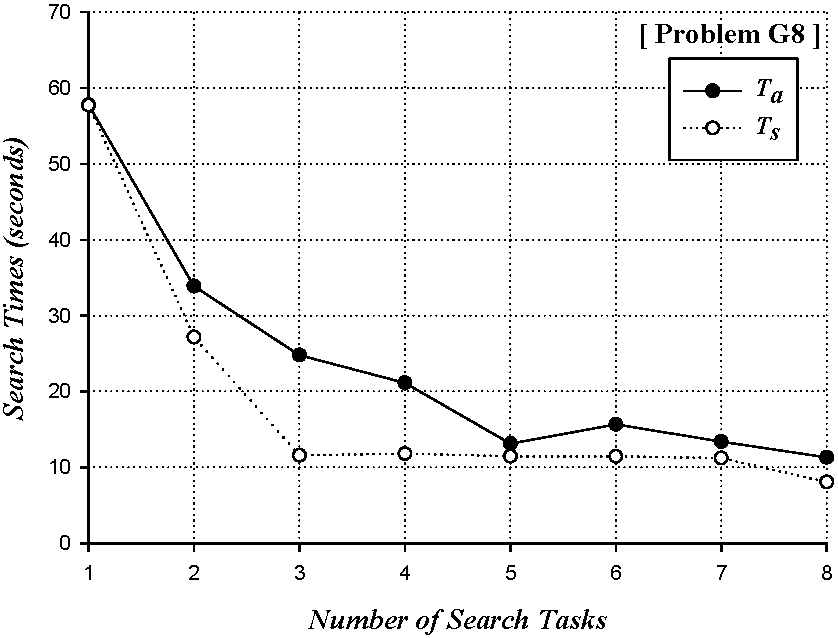
\includegraphics[width=0.65\linewidth]{images/search_times}
	\caption{Exemplo de gráfico.}
	\label{fig:exemplo_de_figura3}
\end{figure}

\subsubsection{Distribuição dos Elementos}
A forma como o texto e outros elementos (tabelas, figuras, etc.) se distribui por uma página, deve ser tal que se evitem grandes blocos vazios no final da página. Embora algumas sistemas de composição tendam a garantir isso automaticamente (como o LaTeX), é costume serem necessárias afinações para resolver, manualmente, essas (e outras) desformatações. No entanto, essas afinações devem ser deixadas para a fase pré-impressão, já com o conteúdo do documento estabilizado, de forma a evitar trabalho inconsequente.


\subsubsection{Correcção Ortográfica}
Para além da qualidade tipográfica do relatório, é imprescindível minimizar (se possível até, erradicar) erros ortográficos. Qualquer sistema de composição de documentos suporta correção ortográfica (e, muitas vezes, sintática), pelo que não é aceitável a submissão para avaliação de relatórios sem revisão ortográfica prévia.


\subsubsection{Referências Bibliográficas}
Ao longo do documento, deve ficar sempre perfeitamente claro o que é escrita original e o que foi baseado (ou até reproduzido de) noutras fontes. 

Todas as fontes devem ser descritas na formatação usada na Bibliografia e referenciadas, no texto, pelos seus identificadores únicos. Por exemplo: ``Uma solução para o problema em causa deve respeitar as propriedades {\it x}, {\it y} e {\it z} \cite{INPROC1}.'', ou ``Neste trabalho explorou-se a API PThreads \cite{TECH01} com o objetivo de $\dots$''.  No modelo em LaTeX, as referências bibliográficas são definidas no ficheiro {\tt libs/refs.bib}, onde existem entradas de diferentes tipos: livro \cite{BOOK01}, artigo de conferência \cite{INPROC1}, relatório técnico \cite{TECH01} e sítio web \cite{FORD11}.

A reprodução fiel de texto de fontes externas deve ser limitada, surgir entre aspas, ligeiramente destacada, e ter apensa a respetiva referência bibliográfica.  Por exemplo:

\begin{quotation}
``Recently, the employment of GPU devices is a key to achieve higher performance for computer systems. On those systems, GPUs are used for general calculation but with extreme parallelism.'' \cite{INPROC1}
\end{quotation}

\subsubsection{Siglas}
Na primeira vez as siglas devem surgir por extenso, sendo resumidas nas vezes seguintes. Por exemplo: ``o curso atual de Engenharia Informática da \gls{ESTiG} foi reformulado em 2015 e, a par com o curso de Informática de Gestão, representa o leque de licenciaturas da área de Informática que a \gls{ESTiG} oferece''. No modelo em LaTeX, as siglas são definidas no ficheiro {\tt acronym.tex}.




\cleardoublepage
\chapter{Contexto e Tecnologias/Ferramentas}\label{cap:conceptual}

Neste capítulo espera-se uma descrição genérica do problema e da área de intervenção: âmbito, conceitos e tecnologia e/ou uma revisão da literatura (``estado da arte''). No caso de um projeto eminentemente prático, devem ser descritas também as ferramentas usadas e a justificação para a sua escolha.

Normalmente, este capítulo é dividido em múltiplas secções, de forma a compartimentar os tópicos abordados, facilitando assim a sua leitura e compreensão.
\cleardoublepage
\chapter{Abordagem/Análise/Modelação}\label{cap:metodology}

Neste capítulo espera-se uma descrição detalhada do problema e da proposta de solução. 

No caso de projetos de desenvolvimento de software, deverá deitar-se mão dos conceitos e ferramentas de Análise/Modelação estudadas durante o curso (por exemplo, diagramas UML ou outra linguagem gráfica). Deve-se indicar explicitamente as tarefas a desempenhar pelo sistema, e os atores que interagem com o mesmo. A descrição deve ter suficiente detalhes  para perceber as dificuldades associadas à resolução do problema.

\cleardoublepage
\chapter{Desenvolvimento/Implementação}\label{cap:development}

Neste capítulo é descrito o trabalho de implementação, salientando os pontos mais relevantes da mesma, dificuldades  encontradas ou soluções técnicas inovadoras desenvolvidas ou aplicadas.  Em particular, se foi usado código desenvolvido por terceiros (por exemplo, código {\it open-source}), deve ser facilmente distinguível quais as funcionalidades originais do mesmo e o que foi necessário implementar para obter as funcionalidades desejadas.

\cleardoublepage
\chapter{Testes/Avaliação/Discussão}\label{cap:test}

Este capítulo apresenta os testes realizados para verificar que o projeto desenvolvido cumpre os objetivos assumidos e resolve, de facto, o problema descrito na Análise/Modelação. 

Para uma melhor compreensão, os resultados de cada teste devem ser precedidos de uma descrição, mesmo que resumida, do teste realizado e dos resultados esperados.

Os resultados do trabalho são comentados, acrescentando-lhe valor:

\begin{itemize}
	\item  O que é que se pode inferir ou conjeturar dos resultados obtidos? 
	\item O que poderia/deveria ter sido feito de forma diferente? 
	\item Onde se foi além dos objetivos iniciais?
	\item  Quais os objetivos que ficaram por cumprir, e porquê ?
\end{itemize}


\cleardoublepage
\chapter{Conclusões}\label{cap:conclusions}

As conclusões devem sintetizar e proporcionar uma perspetiva unificadora ao trabalho efetuado. Poderá ser feita uma breve referência a trabalhos de outros com semelhanças ao efetuado e ao conhecimento que resultou do trabalho efetuado, bem como sugestões de trabalho futuro. A coerência do documento implica que as conclusões devem ser coerentes com as ideias expostas na introdução.

%% estilo de referências. outros valores posíveis são 'plain' e 'abbrv' apalike
%\bibliographystyle{plain}
%% listagem de referências
%\bibliography{lib/refs}

%  Caso seja usado biblatex
\printbibliography


% Apêndices
\appendix

%http://tex.stackexchange.com/questions/59572/custom-page-numbering-for-appendix
\pretocmd{\chapter}{%
	\clearpage
	\pagenumbering{arabic}%
	\renewcommand*{\thepage}{\thechapter\arabic{page}}%
}{}{}

\chapter{Proposta Original do Projeto}
\label{apendice1}

\begin{figure}
%\centering 
\hspace{-12ex}
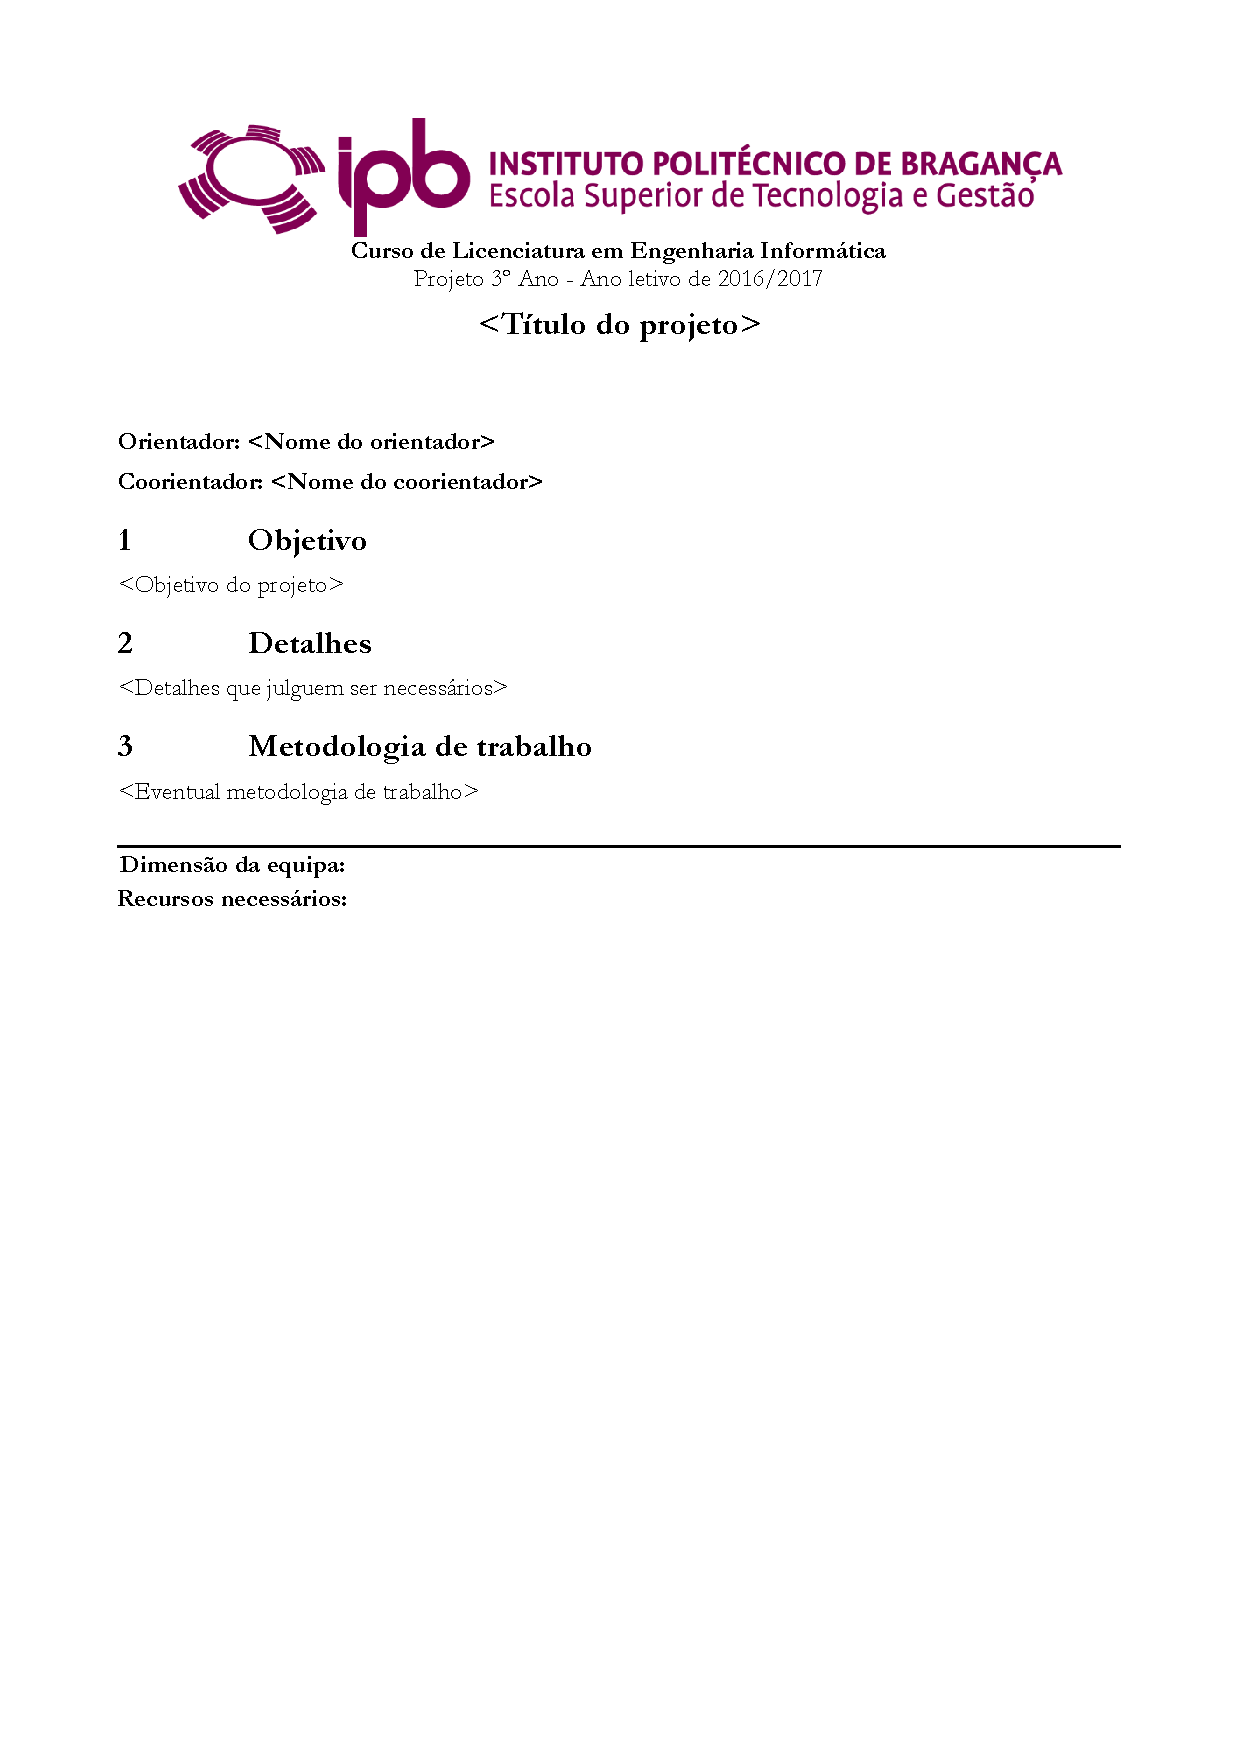
\includegraphics{etc/PropostaProjeto.pdf}
\end{figure}
\chapter{Outro(s) Apêndice(s)}
\label{apendice2}

Listagens de código fonte, texto/imagens produzidos por testes complementares, etc.


\end{document}
